\documentclass{ximera}

 

\usepackage{epsfig}

\graphicspath{
  {./}
  {figures/}
}

\usepackage{morewrites}
\makeatletter
\newcommand\subfile[1]{%
\renewcommand{\input}[1]{}%
\begingroup\skip@preamble\otherinput{#1}\endgroup\par\vspace{\topsep}
\let\input\otherinput}
\makeatother

\newcommand{\includeexercises}{\directlua{dofile("/home/jim/linearAlgebra/laode/exercises.lua")}}

%\newcounter{ccounter}
%\setcounter{ccounter}{1}
%\newcommand{\Chapter}[1]{\setcounter{chapter}{\arabic{ccounter}}\chapter{#1}\addtocounter{ccounter}{1}}

%\newcommand{\section}[1]{\section{#1}\setcounter{thm}{0}\setcounter{equation}{0}}

%\renewcommand{\theequation}{\arabic{chapter}.\arabic{section}.\arabic{equation}}
%\renewcommand{\thefigure}{\arabic{chapter}.\arabic{figure}}
%\renewcommand{\thetable}{\arabic{chapter}.\arabic{table}}

%\newcommand{\Sec}[2]{\section{#1}\markright{\arabic{ccounter}.\arabic{section}.#2}\setcounter{equation}{0}\setcounter{thm}{0}\setcounter{figure}{0}}

\newcommand{\Sec}[2]{\section{#1}}

\setcounter{secnumdepth}{2}
%\setcounter{secnumdepth}{1} 

%\newcounter{THM}
%\renewcommand{\theTHM}{\arabic{chapter}.\arabic{section}}

\newcommand{\trademark}{{R\!\!\!\!\!\bigcirc}}
%\newtheorem{exercise}{}

\newcommand{\dfield}{{\sf dfield9}}
\newcommand{\pplane}{{\sf pplane9}}

\newcommand{\EXER}{\section*{Exercises}}%\vspace*{0.2in}\hrule\small\setcounter{exercise}{0}}
\newcommand{\CEXER}{}%\vspace{0.08in}\begin{center}Computer Exercises\end{center}}
\newcommand{\TEXER}{} %\vspace{0.08in}\begin{center}Hand Exercises\end{center}}
\newcommand{\AEXER}{} %\vspace{0.08in}\begin{center}Hand Exercises\end{center}}

% BADBAD: \newcommand{\Bbb}{\bf}

\newcommand{\R}{\mbox{$\Bbb{R}$}}
\newcommand{\C}{\mbox{$\Bbb{C}$}}
\newcommand{\Z}{\mbox{$\Bbb{Z}$}}
\newcommand{\N}{\mbox{$\Bbb{N}$}}
\newcommand{\D}{\mbox{{\bf D}}}
\usepackage{amssymb}
%\newcommand{\qed}{\hfill\mbox{\raggedright$\square$} \vspace{1ex}}
%\newcommand{\proof}{\noindent {\bf Proof:} \hspace{0.1in}}

\newcommand{\setmin}{\;\mbox{--}\;}
\newcommand{\Matlab}{{M\small{AT\-LAB}} }
\newcommand{\Matlabp}{{M\small{AT\-LAB}}}
\newcommand{\computer}{\Matlab Instructions}
\newcommand{\half}{\mbox{$\frac{1}{2}$}}
\newcommand{\compose}{\raisebox{.15ex}{\mbox{{\scriptsize$\circ$}}}}
\newcommand{\AND}{\quad\mbox{and}\quad}
\newcommand{\vect}[2]{\left(\begin{array}{c} #1_1 \\ \vdots \\
 #1_{#2}\end{array}\right)}
\newcommand{\mattwo}[4]{\left(\begin{array}{rr} #1 & #2\\ #3
&#4\end{array}\right)}
\newcommand{\mattwoc}[4]{\left(\begin{array}{cc} #1 & #2\\ #3
&#4\end{array}\right)}
\newcommand{\vectwo}[2]{\left(\begin{array}{r} #1 \\ #2\end{array}\right)}
\newcommand{\vectwoc}[2]{\left(\begin{array}{c} #1 \\ #2\end{array}\right)}

\newcommand{\ignore}[1]{}


\newcommand{\inv}{^{-1}}
\newcommand{\CC}{{\cal C}}
\newcommand{\CCone}{\CC^1}
\newcommand{\Span}{{\rm span}}
\newcommand{\rank}{{\rm rank}}
\newcommand{\trace}{{\rm tr}}
\newcommand{\RE}{{\rm Re}}
\newcommand{\IM}{{\rm Im}}
\newcommand{\nulls}{{\rm null\;space}}

\newcommand{\dps}{\displaystyle}
\newcommand{\arraystart}{\renewcommand{\arraystretch}{1.8}}
\newcommand{\arrayfinish}{\renewcommand{\arraystretch}{1.2}}
\newcommand{\Start}[1]{\vspace{0.08in}\noindent {\bf Section~\ref{#1}}}
\newcommand{\exer}[1]{\noindent {\bf \ref{#1}}}
\newcommand{\ans}{}
\newcommand{\matthree}[9]{\left(\begin{array}{rrr} #1 & #2 & #3 \\ #4 & #5 & #6
\\ #7 & #8 & #9\end{array}\right)}
\newcommand{\cvectwo}[2]{\left(\begin{array}{c} #1 \\ #2\end{array}\right)}
\newcommand{\cmatthree}[9]{\left(\begin{array}{ccc} #1 & #2 & #3 \\ #4 & #5 &
#6 \\ #7 & #8 & #9\end{array}\right)}
\newcommand{\vecthree}[3]{\left(\begin{array}{r} #1 \\ #2 \\
#3\end{array}\right)}
\newcommand{\cvecthree}[3]{\left(\begin{array}{c} #1 \\ #2 \\
#3\end{array}\right)}
\newcommand{\cmattwo}[4]{\left(\begin{array}{cc} #1 & #2\\ #3
&#4\end{array}\right)}

\newcommand{\Matrix}[1]{\ensuremath{\left(\begin{array}{rrrrrrrrrrrrrrrrrr} #1 \end{array}\right)}}

\newcommand{\Matrixc}[1]{\ensuremath{\left(\begin{array}{cccccccccccc} #1 \end{array}\right)}}



\renewcommand{\labelenumi}{\theenumi)}
\newenvironment{enumeratea}%
{\begingroup
 \renewcommand{\theenumi}{\alph{enumi}}
 \renewcommand{\labelenumi}{(\theenumi)}
 \begin{enumerate}}
 {\end{enumerate}\endgroup}



\newcounter{help}
\renewcommand{\thehelp}{\thesection.\arabic{equation}}

%\newenvironment{equation*}%
%{\renewcommand\endequation{\eqno (\theequation)* $$}%
%   \begin{equation}}%
%   {\end{equation}\renewcommand\endequation{\eqno \@eqnnum
%$$\global\@ignoretrue}}

%\input{psfig.tex}

\author{Martin Golubitsky and Michael Dellnitz}

%\newenvironment{matlabEquation}%
%{\renewcommand\endequation{\eqno (\theequation*) $$}%
%   \begin{equation}}%
%   {\end{equation}\renewcommand\endequation{\eqno \@eqnnum
% $$\global\@ignoretrue}}

\newcommand{\soln}{\textbf{Solution:} }
\newcommand{\exercap}[1]{\centerline{Figure~\ref{#1}}}
\newcommand{\exercaptwo}[1]{\centerline{Figure~\ref{#1}a\hspace{2.1in}
Figure~\ref{#1}b}}
\newcommand{\exercapthree}[1]{\centerline{Figure~\ref{#1}a\hspace{1.2in}
Figure~\ref{#1}b\hspace{1.2in}Figure~\ref{#1}c}}
\newcommand{\para}{\hspace{0.4in}}

\renewenvironment{solution}{\suppress}{\endsuppress}

\ifxake
\newenvironment{matlabEquation}{\begin{equation}}{\end{equation}}
\else
\newenvironment{matlabEquation}%
{\let\oldtheequation\theequation\renewcommand{\theequation}{\oldtheequation*}\begin{equation}}%
  {\end{equation}\let\theequation\oldtheequation}
\fi

\makeatother


\title{m10.tex}

\begin{document}
\begin{abstract}
BADBAD
\end{abstract}
\maketitle

\chapter{Orthogonality}

\subsection*{Section~\protect{\ref{S:orthonormal}} Orthonormal Bases}
\rhead{S:orthonormal}{ORTHONORMAL BASES}

\exer{c7.4.1}
\ans The vectors $w_1 = \frac{1}{\sqrt{3}}(1,1,-1)$ and
$w_2 = \frac{1}{\sqrt{2}}(0,1,1)$ form an orthonormal basis
for the solution set.

\soln Find one vector which is a solution to the equation, for
example $(1,1,-1)$.  Then, divide the vector by its length, obtaining
the unit vector $w_1$.  By inspection, find a vector $v_2$ which
satisfies both the given equation and $w_1 \cdot v_2 = 0$.  Then set
$w_2 = \frac{1}{||v_2||}v_2$.

\exer{c7.4.2}
(a) By Theorem~\ref{T:orthocoord}:
\[
[v]_{\cal V} = (v \cdot v_1, v \cdot v_2) = 
\frac{1}{\sqrt{5}}(9,-2).
\]

(b) By \Ref{e:coordorthomat}:
\[ [A]_{\cal V} = \mattwo{Av_1 \cdot v_1}{Av_2 \cdot v_1}
{Av_1 \cdot v_2}{Av_2 \cdot v_2} = \mattwo{-1}{3}{2}{-1}. \]

%\exer{c7.4.3} No written solution necessary.


\subsection*{Section~\protect{\ref{S:LSA}} Least Squares Approximations}
\rhead{S:LSA}{LEAST SQUARES APPROXIMATIONS}

\exer{c7.5.1}
\ans The vectors $v_1 = \frac{1}{5}(3,4)$ and $v_2 = \frac{1}{5}(-4,3)$
form an orthonormal basis for $\R^2$.

\soln Find these vectors using Gram-Schmidt orthonormalization
(Theorem~\ref{T:orthobasis}).  More
specifically, calculate $v_1$ and $v_2$ such that:
\[
\begin{array}{rcl}
v_1 & = & \frac{1}{||w_1||}w_1 = \frac{1}{5}(3,4). \\
v_2' & = & w_2 - (w_2 \cdot v_1)v_1 = (1,5) - \frac{23}{25}(3,4)
= \frac{1}{25}(-44,33). \\
v_2 & = & \frac{1}{||v_2'||}v_2' = \frac{5}{11}
\left(\frac{1}{25}(-44,33)\right) = \frac{1}{5}(-4,3).
\end{array}
\]

\exer{c7.5.2}
\ans The vectors $v_1 = \frac{1}{\sqrt{14}}(1,2,3)$ and
$v_2 = \frac{1}{\sqrt{4746}}(19,52,-41)$ form an orthonormal basis
for $W$.

\soln Use Gram-Schmidt orthonormalization
(Theorem~\ref{T:orthobasis}) to calculate $v_1$ and $v_2$ such that:
\[
\begin{array}{rcl}
v_1 & = & \frac{1}{||w_1||}w_1 = \frac{1}{\sqrt{14}}(1,2,3). \\
v_2' & = & w_2 - (w_2 \cdot v_1)v_1 = (2,5,-1) -
\frac{9}{14}(1,2,3) = \frac{1}{14}(19,52,-41). \\
v_2 & = & \frac{1}{||v_2'||}v_2' = \frac{14}{\sqrt{4746}}
\left(\frac{1}{14}(19,52,-41)\right) = \frac{1}{\sqrt{4746}}
(19,52,-41).
\end{array}
\]

\exer{c7.5.3}
By Corollary~\ref{c:extendindependent},
a linearly independent subset of $\R^n$ can be extended to form a
basis for $\R^n$ by adding linearly independent vectors
$v_{k+1},\ldots,v_n$ which are not in the span of
$\{w_1,\ldots,w_k\}$.  Then, Gram-Schmidt orthonormalization
(Theorem~\ref{T:orthobasis}) can be used
to form the orthonormal basis $\{w_1,\ldots,w_n\}$ from the basis
$\{w_1,\ldots,w_k,v_{k+1},\ldots,v_n\}$.

\exer{c7.5.4}
\ans
An orthonormal basis for the subspace spanned by {\tt w1}, {\tt w2},
and {\tt w3} is:
\begin{verbatim}
v1 = (0.2132, 0.1066, 0.3198, 0.5330, 0.7462)
v2 = (0.2236, -0.3927, 0.8399, -0.1978, -0.2265)
v3 = (0.8452, -0.3542, -0.3979, -0.0409, 0.0088)
\end{verbatim}
Adding the vectors
\begin{verbatim}
v4 = (0.4340, 0.8222, 0.1827, 0, -0.3198)
v5 = (0.0424, 0.1813, 0.0251, -0.8217, 0.5381)
\end{verbatim}
to this basis forms an orthonormal basis for $\R^5$.

\soln The following set of \Matlab commands computes {\tt v1}, {\tt v2},
and {\tt v3} by Gram-Schmidt orthonormalization:
\begin{verbatim}
v1 = 1/norm(w1)*w1;
v2p = w2 - dot(w2,v1)*v1;
v2 = 1/norm(v2p)*v2p;
v3p = w3 - dot(w3,v1)*v1 - dot(w3,v2)*v2;
v3 = 1/norm(v3p)*v3p;
\end{verbatim}
We can verify this result by creating the matrix {\tt A} whose columns
are {\tt w1'}, {\tt w2'}, and {\tt w3'}, then using the command
{\tt [Q R] = qr(A,0)}.

\para We extend the basis by finding a vector {\tt w4} which is
orthogonal to {\tt w1}, {\tt w2}, and {\tt w3}.  That is, solve the
linear system
\[
\vecthree{{\tt w1}}{{\tt w2}}{{\tt w3}}{\tt w4'} = \vecthree{0}{0}{0}. \]
One possible solution is {\tt w4} $= (19,36,8,0,-14)$.  Then, find
the unit vector {\tt v4} in the direction of {\tt w4}.  Next, add a
fifth basis vector by finding the vector {\tt w5} which is orthogonal
to {\tt \{w1,w2,w3,w4\}}.  In this case, {\tt w5}
$= (22,94,13,-426,279)$.  Normalize this vector to obtain {\tt v5}.


\newpage
\subsection*{Section~\protect{\ref{S:7.6}} Least Squares Fitting of Data}
\rhead{S:7.6}{LEAST SQUARES FITTING OF DATA}

\exer{c7.6.1}
(a) \ans The best linear fit to the data is obtained with $m \approx
0.4084$ and $b \approx 0.9603$, where $m$ and $b$ are measured in
billions.

\soln Create the matrix $A$ whose columns are $w_1$ and $w_2$.  Then use
\Ref{E:nearestvector} to compute the best values for $m$ and $b$.

(b) In 1910, $P \approx 408.4(1) + 960.3 = 1369$ million people.

\para In 2000, $P \approx 408.4(10) + 960.3 = 5044$ million people.

(c) \ans The prediction for 2000 is likely to be low.

\soln As shown in Figure~\ref{c7.6.1}, a linear approximation does not
fit the data points well.  To understand why, assume that population
change is governed by the differential equation:
\[
\frac{dP}{dT} = rP
\]
where $r$ is constant.  Then $\frac{d^2P}{dT^2} = r^2P > 0$.
Then the population curve is concave up, and a linear approximation
underestimates the population at the endpoints of the curve.

\begin{figure}[htb]
		\centerline{%
		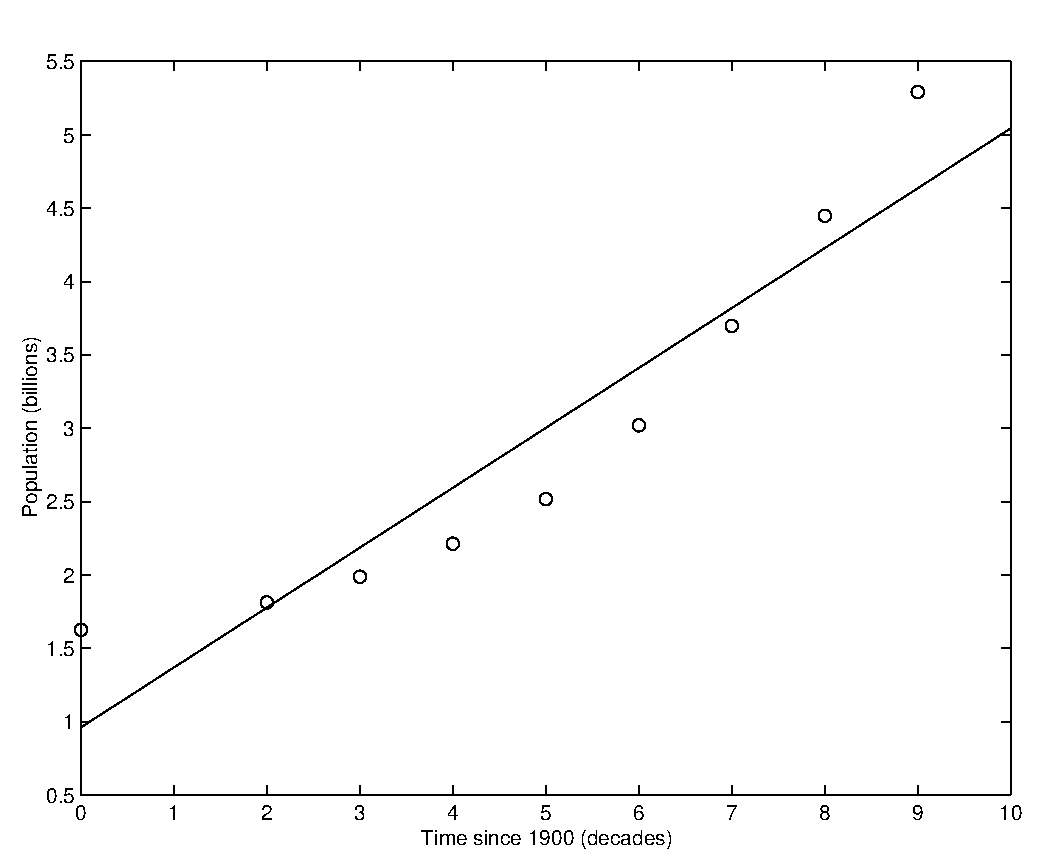
\psfig{file=exfigure/7-6-1.eps,width=3.0in}}
	\exercap{c7.6.1}
\end{figure}

\exer{c7.6.2}
\ans A good sinusoidal approximation for the low temperatures in Paris
is 
\[ \hbox{temp}(t) = 51.4167 - 9.4908\cos(\frac{2\pi t}{12}) -
8.4745\sin(\frac{2\pi t}{12}). \]
An approximation for the low temperatures in Rio is
\[ \hbox{temp}(t) = 67.8333 + 3.3987\cos(\frac{2\pi t}{12}) +
3.5654\sin(\frac{2\pi t}{12}). \]

\soln Use a set of \Matlab commands similar to those shown in
Section~\ref{S:7.6} to graph the low temperatures in Paris
(Figure~\ref{c7.6.2}a) and Rio (Figure~\ref{c7.6.2}b).  The
variations about the mean temperature are $d_P = 12.7237$ and
$d_R = 4.9258$.  (These values can be computed for each set of data
by typing {\tt d = sqrt(b(2)\^{}2 + b(3)\^{}2)} in \Matlabp.) 
The low temperatures in Paris vary more depending on the time of
year than do the temperatures in Rio, which is consistent with
the graphs and with the values of $d$ for the high temperatures.

\begin{figure}[htb]
		\centerline{%
		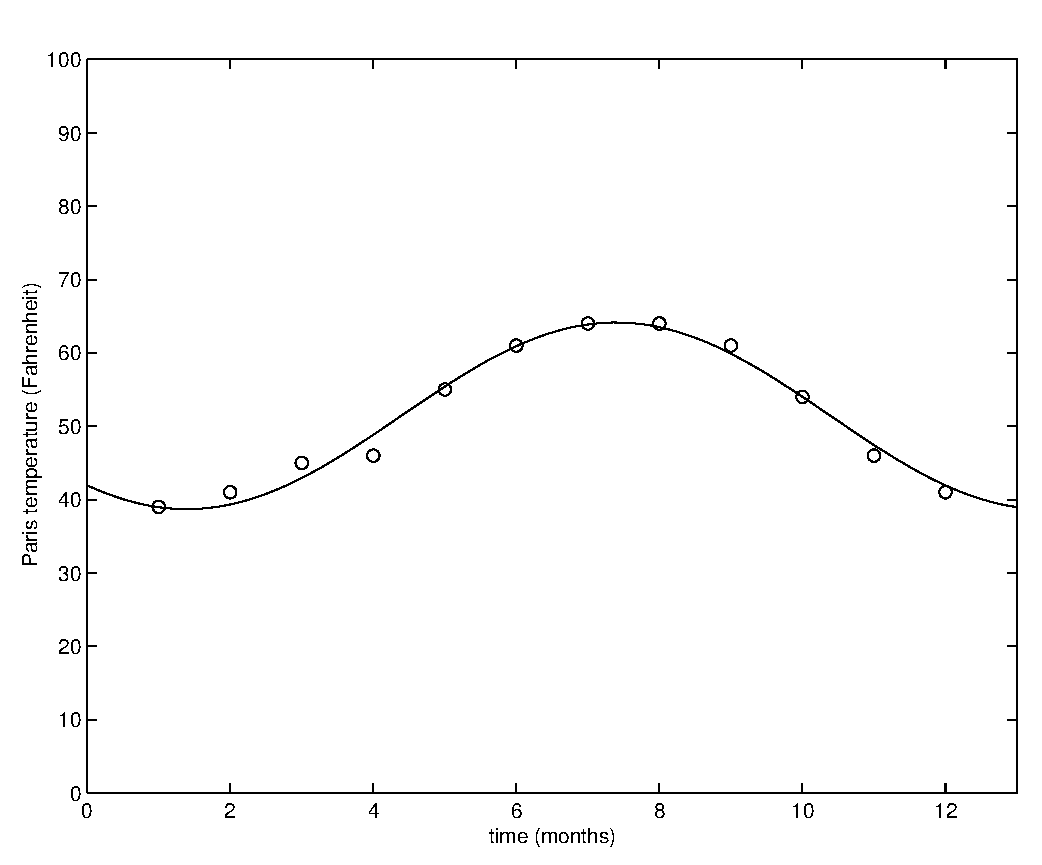
\psfig{file=exfigure/7-6-2a.eps,width=2.75in}
		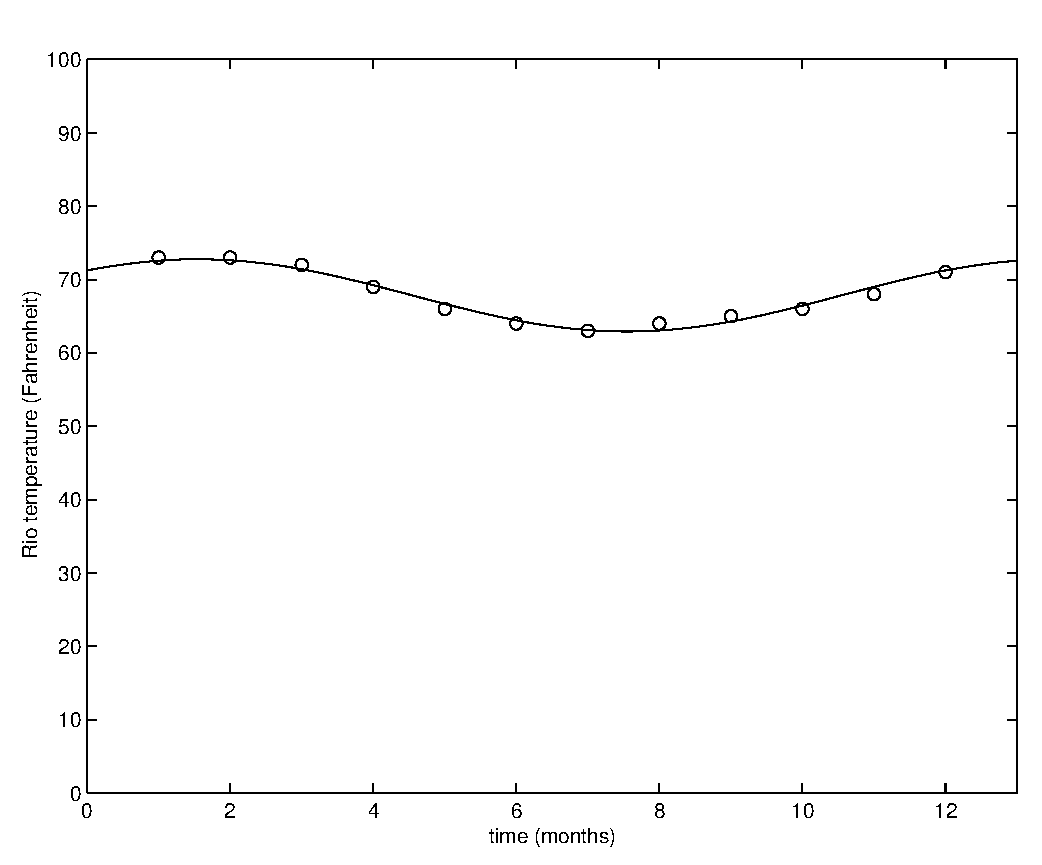
\psfig{file=exfigure/7-6-2b.eps,width=2.75in}}
	\exercaptwo{c7.6.2}
\end{figure}

\exer{c7.6.3}
\ans Let $R$ be the number of days in the year with precipitation and
let $s$ be the percentage of sunny hours to daylight hours.  Then the
best linear estimate of the relationship between the two is:
\[ R \approx 199.2 - 156.6s. \]

\soln In \Matlabp, enter the data for number of rainy days as the vector
$R$, and then enter the data for percentage of sunny hours as the vector
$s_1$.  Then create the $1 \times 10$ vector $s_2 = (1,1,\dots,1)$.  Now,
find the best vector $b = (b_1,b_2)$ such that $R = b_1s_1 + b_2s_2$. 
This vector can be found using \Ref{E:nearestvector}.  The solution vector
is $(b_1,b_2) \approx (-156.6,199.2)$.  Figure~\ref{c7.6.3} shows the
actual data graphed against the linear estimate.

\begin{figure}[htb]
		\centerline{%
		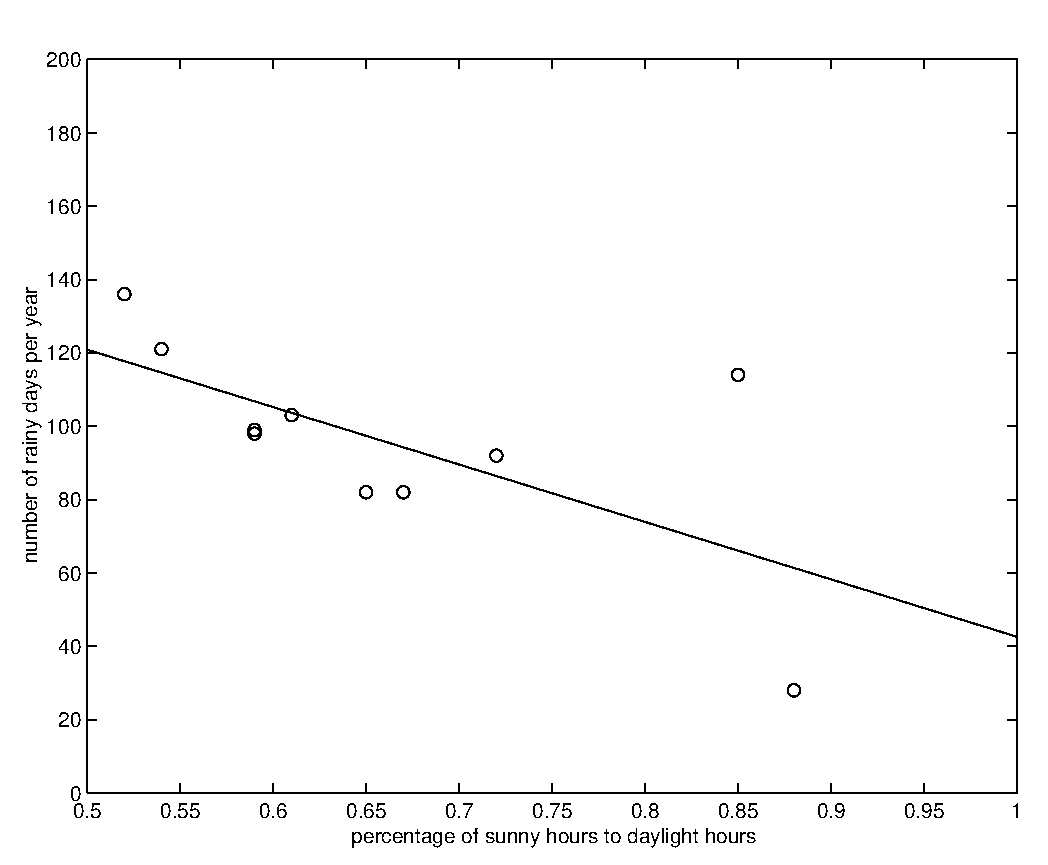
\psfig{file=exfigure/7-6-3.eps,width=3.0in}}
	\exercap{c7.6.3}
\end{figure}


\subsection*{Section~\protect{\ref{S:symmetric}} Symmetric Matrices}
\rhead{S:symmetric}{SYMMETRIC MATRICES}

\exer{c7.7.1}
(a) We can calculate the discriminant $D$ of matrix $A$ using
\Ref{e:discriminant}:
\[ D = \trace(A)^2 - 4\det(A) = (a + d)^2 - 4(ad - b^2) =
a^2 + 2ad + b^2 - 4ad + 4b^2 = (a - d)^2 + 4b^2. \]
Therefore, $D \geq 0$ for all real symmetric matrices $A$.  The
eigenvalues of $A$ are
\[ \lambda_1 = \frac{(a + d) + \sqrt{D}}{2} \AND
\lambda_2 = \frac{(a + d) - \sqrt{D}}{2}. \]
Thus, $\lambda_1$ and $\lambda_2$ are real since $D$ is non-negative.

(b) Matrix $A$ has equal eigenvalues only if $D = 0$.  According to
the computation in (a) of this problem, $D = 0$ only if $a = d$ and
$b = 0$.  Therefore, if $\lambda_1 = \lambda_2$, then $A$ is a
multiple of $I_2$.

\exer{c7.7.2}
\ans The eigenvalues of $A$ are $\lambda_1 = 2$ and $\lambda_2 = -3$,
with respective eigenvectors $v_1 = (2,1)$ and $v_2 = (1,-2)$.

\soln Indeed, $v_1 \cdot v_2 = (2,1) \cdot (1,-2) = 0$, so the
eigenvectors are orthogonal.

\exer{exer:powita}
\ans The eigenvectors of $A$ are $w_1 = (1,1)$ and
$w_2 = (1,-1)$ with eigenvalues $\lambda_1 = 4$ and $\lambda_2 = -2$.  

\soln Note that any matrix of the form $\mattwo{a}{b}{b}{a}$
has eigenvectors $w_1$ and $w_2$ with eigenvalues
$\lambda_1 = a + b$ and $\lambda_2 = a - b$.
By iterating using {\tt map}, we see that $v_j$ approaches a multiple
of $(1,1)$ as $j$ increases for $v_0 \neq (1,-1)$.  If $v_0$ is a
multiple of $(1,-1)$, then $v_j$ is a multiple of $(1,-1)$ for all $j$.

\para In Exercises~\ref{exer:powita} -- \ref{exer:powitc} let $u_1$ be the
eigenvector of matrix associated to the eigenvalue $\lambda_1$ where
$|\lambda_1| > |\lambda_2|$. These exercises demonstrate that $v_j$ 
approaches the direction of $u_1$ as $j$ increases when $v_0$ is
not a scalar multiple of $u_2$.

\exer{exer:powitb}
\ans The eigenvectors of $B$ are $w_1 = (1,1)$ and $w_2 = (1,-1)$ with  
eigenvalues $\lambda_1 = 20$ and $\lambda_2 = 2$.  

\soln See solution to Exercise~\ref{exer:powita}.

\exer{exer:powitc}
\ans The eigenvectors of $C$ are $w_1 = (1,1)$ and $w_2 = (1,-1)$ with 
eigenvalues $\lambda_1 = -2$ and $\lambda_2 = 2.01$.  

\soln See comment after the solution to Exercise~\ref{exer:powita}.
By iterating using {\tt map}, we see that $v_j$ approaches a multiple
of $(1,-1)$ as $j$ increases for $v_0 \neq (1,1)$.  If $v_0$ is a
multiple of $(1,1)$, then $v_j$ is a multiple of $(1,1)$ for all $j$.

\exer{c7.7.3}
In this case, for any vector $v_0 = (x,y)$, the result of the iteration
is $v_1 = Av_0 = 2(y,x)$.  That is, any vector multiplied by $A$ is
reflected across the line $y = x$ and doubled in length.  The result
is different from that in Exercises~\ref{exer:powita} -- \ref{exer:powitc}
because the eigenvalues are $\lambda_1 = 2$ and $\lambda_2 = -2$, so
$|\lambda_1| = |\lambda_2|$.


\subsection*{Section~\protect{\ref{S:QR}} Orthogonal Matrices and $QR$
Decomposition}
\rhead{S:QR}{ORTHOGONAL MATRICES AND $QR$ DECOMPOSITION}

\exer{c7.9.1a} \ans The matrix is not orthogonal.

\soln By Lemma~\ref{lem:orthprop}, a matrix
$A$ is orthogonal if and only if $A^tA = I_n$.
\[
\mattwo{2}{0}{0}{1}\mattwo{2}{0}{0}{1} = \mattwo{4}{0}{0}{1} \neq I_2.
\]

\exer{c7.9.1b} \ans The matrix is orthogonal, since
\[
\matthree{0}{0}{1}{1}{0}{0}{0}{1}{0}
\matthree{0}{1}{0}{0}{0}{1}{1}{0}{0} =
I_3.
\]

\exer{c7.9.1c} The matrix is orthogonal, since
\[
\matthree{0}{0}{-1}{-1}{0}{0}{0}{1}{0}
\matthree{0}{1}{0}{0}{0}{-1}{-1}{0}{0} =
I_3.
\]

\exer{c7.9.1d} The matrix is orthogonal, since
\[
\mattwo{\cos(1)}{\sin(1)}{-\sin(1)}{\cos(1)}
\mattwo{\cos(1)}{-\sin(1)}{\sin(1)}{\cos(1)}
= I_2.
\]

\exer{c7.9.1e} The matrix is not orthogonal, since all orthogonal matrices
are square.

\exer{c7.9.2}
For this proof, we use the fact that, if $C$ is a complex matrix, then
$(Cv) \cdot w = v \cdot (\overline{C}^tw)$.  This was shown in the discussion
of Hermitian inner products in Section~\ref{S:symmetric}.  In particular,
since $Q$ is a real matrix, $(Qv) \cdot w = v \cdot (Q^tw)$.  Therefore,
since $Q$ is orthogonal:
\[
||Qv||^2 = (Qv) \cdot (Qv) = (Q^tQv) \cdot v = (I_nv) \cdot v
= v \cdot v = ||v||^2.
\]

\newpage
\exer{c7.9.3a}
$H = I_2 - \dps\frac{2}{2}\vectwo{1}{1}\left(\begin{array}{rr} 1 & 1
\end{array}\right) = \mattwo{1}{0}{0}{1} - \mattwo{1}{1}{1}{1}
= \mattwo{0}{-1}{-1}{0}.$

\exer{c7.9.3b}
$H = I_2 - \dps\frac{2}{4}\mattwo{0}{0}{0}{4} =
\mattwo{1}{0}{0}{-1}$.

\exer{c7.9.3c}
$H = I_3 - \dps\frac{2}{27}\matthree{1}{-1}{-5}{-1}{1}{5}{-5}{5}{25}
= \frac{1}{27}\matthree{25}{2}{10}{2}{25}{-10}{10}{-10}{-50}$.

\exer{c7.9.3d}
$H = I_4 - \dps\frac{2}{21}\left(\begin{array}{rrrr} 1 & 0 & 4 & -2 \\
0 & 0 & 0 & 0 \\ 4 & 0 & 16 & -8 \\ -2 & 0 & -8 & 4 \end{array}\right)
= \frac{1}{21}\left(\begin{array}{rrrr} 19 & 0 & -8 & 4 \\
0 & 21 & 0 & 0 \\ -8 & 0 & -9 & 16 \\ 4 & 0 & 16 & 13
\end{array}\right)$.

\exer{c7.9.4}
\ans The matrix that reflects the plane across $(1,2)$ is
\[
H = \mattwo{-\frac{3}{5}}{\frac{4}{5}}{\frac{4}{5}}{\frac{3}{5}}.
\]

\soln The matrix that reflects the plane across $(1,2)$ is the
Householder matrix associated to the vector $u$, where $u \cdot (1,2)
= 0$.  Compute $H$, the Householder matrix associated to $u = (2,-1)$.

\exer{c7.9.45}
Let $A$ be an orthogonal matrix.  By
Definition~\ref{def:orthmat}, the columns of $A$ form an orthonormal
basis for $\R^n$.  We must show that the rows of $A$ also form an
orthonormal basis for $\R^n$.  By Lemma~\ref{lem:orthprop}(b), $A^t =
A^{-1}$.  From this, we can show
\[
I_n = AA^{-1} = AA^t = (A^t)^t(A^t).
\]
Thus, by Lemma~\ref{lem:orthprop}(a), $A^t$ is an orthogonal matrix;
so the columns of $A^t$, which are the rows of $A$, form an orthonormal
basis for $\R^n$.

\exer{c7.5.5a}
The orthonormal basis generated by the command {\tt [Q R] = qr(A,0)} is:
\begin{verbatim}
v1 =          v2 =
   -0.7071        0.7071
    0.7071        0.7071
\end{verbatim}

\exer{c7.5.5b}
The orthonormal basis generated by the command {\tt [Q R] = qr(A,0)} is:

\begin{verbatim}
v1 =          v2 =
   -0.2673        0.0514
    0.5345       -0.8230
   -0.8018       -0.5658
\end{verbatim}

\exer{c7.5.5c}
The orthonormal basis generated by the command {\tt [Q R] = qr(A,0)} is:
\begin{verbatim}
v1 =          v2 =          v3 = 
   -0.2673        0.0514       -0.9623
    0.5345       -0.8230       -0.1925
   -0.8018       -0.5658        0.1925
\end{verbatim}

\exer{c7.5.5d}
The orthonormal basis generated by the command {\tt [Q R] = qr(A,0)} is:

\begin{verbatim}
v1 =          v2 =          v3 = 
   -0.4082        0.6882        0.0190
         0       -0.2294       -0.8494
    0.8165        0.4588       -0.2282
         0        0.4588        0.0127
    0.4082       -0.2294        0.4754
\end{verbatim}

\exer{c7.5.6}
\ans
\begin{verbatim}
H1 =                                   H2 =
   0.6245  -0.7220  -0.2744   0.1155      0.2807   0.6679  -0.3083  -0.6165
  -0.7220  -0.3885  -0.5276   0.2222      0.6679   0.3798   0.2862   0.5725
  -0.2744  -0.5276   0.7995   0.0844     -0.3083   0.2862   0.8679  -0.2642
   0.1155   0.2222   0.0844   0.9645     -0.6165   0.5725  -0.2642   0.4716

H =
   -0.2935    0.1305   -0.6678   -0.6714
   -0.4365   -0.6536   -0.4053    0.4669
   -0.7279   -0.1065    0.6051   -0.3043
   -0.4398    0.7378   -0.1536    0.4885
\end{verbatim}

\soln Find $H_1$ in \Matlab by typing
\begin{verbatim}
H1 = eye(4) - 2/(u1'*u1)*u1*u1'
\end{verbatim}

Calculate $H_2$ similarly.  Confirm that $H = H_1H_2$ is orthogonal by
computing the product $H^tH$ to see that it is $I_4$.
\end{document}
